%!TeX encoding = ISO-8859-1
\documentclass[12pt,a4paper,english
%,twoside,openright
]{tutthesis}
%\documentclass[12pt,a4paper,finnish]{tutthesis}

\usepackage{mathtools}
\usepackage{listings}
\usepackage{caption}
\usepackage{graphicx}
\graphicspath{ {images/} }
\usepackage{lmodern}

% Note that you must choose either Finnish or English here and there in this
% file.
% Other options for document class
  % ,twoside,openright   % If printing on both sides (>80 pages)
  % ,twocolumn           % Can be used in lab reports, not in theses

% Ensure the correct Pdf size (not needed in all environments)
\special{papersize=210mm,297mm}

%
% Define your basic information
%
\author{Jonne Petteri Pihlanen}
\title{Building a Recommendation Engine with Apache Spark}      % primary title (for front page)
\titleB{Suosittelijaj�rjestelm�n rakentaminen Apache Sparkilla} % translated title for abstract
\thesistype{Master of Science thesis} % or Bachelor of Science, Laboratory Report... 
\examiner{????} % without title Prof., Dr., MSc or such

% Special trick to use internal macros outside the cls file
% (e.g. \@author). Trick is reversed with \makeatother a bit later.
\makeatletter

% Define the pdf document properties.  Fill in your own keywords.
\hypersetup{   
  pdftitle={\@title},
  pdfauthor={\@author},
  pdfkeywords={recommmendation}
}


% Put your thesis' main language last
% http://mirrors.ctan.org/macros/latex/required/babel/base/babel.pdf
% !!! 2014-11-03 Second language seems to mess up figure and table
% !!! captions. Do not use it after all (ES)
%%\usepackage[finnish,english]{babel}
%\usepackage[finnish]{babel}
\usepackage[english]{babel}

% You can also add your own commands
\newcommand\todo[1]{{\color{red}!!!TODO: #1}} % Remark text in braces appears in red
\newcommand{\angs}{\textsl{\AA}}              % , e.g. slanted symbol for �ngst�m

% Preparatory content ends here

\pagenumbering{Roman}
\pagestyle{headings}
\begin{document}

%
% Create the title page.
% First the logo. Check its language.
\thispagestyle{empty}
%\vspace*{-.5cm}\noindent
\vspace*{-1cm}\noindent

\includegraphics[width=8cm]{tty_tut_logo}   % Bilingual logo

% Then lay out the author, title and type to the center of page.
\vspace{6.8cm}
\maketitle
\vspace{7cm} % modify if thesis title needs many lines

% Last some additional info to the bottom-right corner
\begin{flushright}  
  \begin{minipage}[c]{6.8cm}
    \begin{spacing}{1.0}
      \textsf{Examiner: \@examiner}\\
      \textsf{Examiner and topic approved by the}\\ 
      \textsf{Faculty Council of the Faculty of}\\
      \textsf{xxxx}\\
      \textsf{on 1st September 2014}\\
    \end{spacing}
  \end{minipage}
\end{flushright}

% Leave the backside of title page empty in twoside mode
\if@twoside
\clearpage
\fi

%
% Use Roman numbering i,ii,iii... for the first pages (abstract, TOC,
% termlist etc)
\pagenumbering{roman} 
\setcounter{page}{0} % Start numbering from zero because command 'chapter*' does page break


% Some fields in abstract are automated, namely those with \@ (author,
% title in the main language, thesis type, examiner).

% !!! Problems with other language. Disable it (ES, 2014-11-03)
%%\begin{otherlanguage}{english} %  Following text in in 2nd language
\chapter*{Abstract}

\begin{spacing}{1.0}
         {\bf \textsf{\MakeUppercase{\@author}}}: \@title\\   % use \@titleB when thesis is in Finnish
         \textsf{Tampere University of Technology}\\
         \textsf{\@thesistype, xx pages} \\
         \textsf{September 2016}\\
         \textsf{Master's Degree Program in Signal Processing}\\
         \textsf{Major: Data Engineering}\\
         \textsf{Examiner: \@examiner}\\
         \textsf{Keywords: }\\
\end{spacing}

The amount of recommendation engines around the Internet is constantly growing.

This paper studies the usage of Apache Spark when building a recommendation engine.


%%\end{otherlanguage} % End on 2nd language part -- (Disabled 2014-11-03)


% Foreign students do not need Fininsh abstract (tiivistelm�). Move
% this before English abstract if thesis is in Finnish. 

% !!! Problems with other language. Disable it (ES, 2014-11-03)
%%\begin{otherlanguage}{finnish} %  Following text in in 2nd language
\chapter*{Tiivistelm�}         % Asterisk * turns numbering off

\begin{spacing}{1.0}
         {\bf \textsf{\MakeUppercase{\@author}}}: \@titleB\\  % or use \@title when thesis is in Finnish
         \textsf{Tampereen teknillinen yliopisto}\\
         \textsf{Diplomity�, xx sivua}\\ %
         \textsf{syyskuu 2016}\\
         \textsf{Signaalink�sittelyn koulutusohjelma}\\
         \textsf{P��aine: Data Engineering}\\
         \textsf{Tarkastajat: \@examiner}\\
         \textsf{Avainsanat: }\\
\end{spacing}


%%\end{otherlanguage} % End on 2nd language part -- (Disabled 2014-11-03)

\makeatother % Make the @ a special symbol again, as \@author and \@title are not neded after this


\chapter*{Preface}

ASDASDASDASDASD


~ 
% Tilde ~ makes an non-breakable spce in LaTeX. Here it is used to get
% two consecutive paragraph breaks

Tampere, 

~


Jonne Pihlanen




%
% Add the table of contents, optionally also the lists of figures,
% tables and codes.
%

\renewcommand\contentsname{Table of Contents} % Set English name (otherwise bilingual babel might break this), 2014-09-01
%\renewcommand\contentsname{Sis�llys}         % Set Finnish name
\setcounter{tocdepth}{3}                      % How many header level are included
\tableofcontents                              % Create TOC

%\renewcommand\lstlistlistingname{List of Programs}      % Set English name (otherwise bilingual babel might break this)
%%\renewcommand\lstlistlistingname{Ohjelmaluettelo} % SetFinnish name, remove this if using English
%\lstlistoflistings                                % Optional: create the list of program codes
%\markboth{}{}                                     % no headers


%
% Term and symbol exaplanations use a special list type
%

\chapter*{List of abbreviations and symbols}
\markboth{}{}                                % no headers

% You don't have to align these with whitespaces, but it makes the
% .tex file more readable
\begin{termlist}
	\item [Recommendation Engine]	System that tries to predict the items that a user woud like
	\item [Collaborative]			Users collaborate with each other to recommend items
	\item [Spark] 					Fast and general engine for large-scale data processing
	\item [Information retrieval (IR)]	Activity of obtaining relevant information resources from a collection of information resources.
	\item [SDK] Software Development Kit
\end{termlist}

% Leave the backside of abbreviation list empty in twoside mode
\cleardoublepage

% The actual text begins here and page numbering changes to 1,2...
\newpage             % needed for page numbering
\pagenumbering{arabic}
\setcounter{page}{1} % Start numbering from zero because command
                     % 'chapter*' does page break
\renewcommand{\chaptername}{} % This disables the prefix 'Chapter' or
                              % 'Luku' in page headers (in 'twoside'
                              % mode)

\chapter{Introduction}
\label{ch:intro} 
% \label{...} allows cross-referencing, e.g. 'as explained in
% Chapter~\ref{ch:intro}' Note that you may have to run the command
% 'latex' or 'pdflatex' twice to get cross-references correctly.  You
% can add labels e.g. to chapters, sections, figures, tables, and
% equations.

Recommender systems have been successfully utilized to aid customers in decision making. In fact, they are constantly present in our everyday life. Whether a customer is shopping online, watching a movie from Netflix, browsing the Facebook or simply reading the news. All of these tasks involve a presence of a recommendation engine. Basically all parts of our daily life include recommendations of some sorts. However, the most basic type of recommendation is the one from human to human and happens completely without computers.

Recommendation can be divided into two major categories: item based and user based.

%Present state of recommendation is to incorporate context awareness into recommendation. Context and Context Aware Recommendation Systems (CARS) are described in Chapter 2.

This thesis is structured as follows. Chapter 2 describes recommendation systems. In Chapter 3, the data for this project and related tasks are discussed. Chapter 4 discusses Apache Spark, an open source framework for building distributed programs. Chapter 5 discusses the results. Finally, in Chapter 6 the evaluation is presented along with conclusions.

%Bigger companies have also released directly and indirectly their open source recommendation solutions. Twitter contributed to Spark project directly by releasing the DIMSUM algorithm, short for Dimension Independent Matrix Square using MapReduce, which limits the list of potential combinations to a reasonable number, enabling other recommendation algorithms to run in a reasonable amount of time \cite{harris14}. Netflix contributed indirectly by hosting the Netflix Prize competitions. Around these competitions, Alternating Least Squares (ALS) algorithm became popular and the ALS implementation in Spark MLlib is inspired by some of the solutions in the competition \cite{ryza15}. DIMSUM and ALS are described in chapter 5.

\chapter{Recommendation Systems}
\label{ch:rs}

Recommendation denotes a task in which items are recommended to users. The most simple version of recommendation is from peer to peer, completely without computers. However, humans can only recommend effectively those items they have personally experienced. This is where recommendation systems (RSs) become useful as they can potentially offer recommendations from thousands of different items. Recommender systems are a set of techniques and software tools that provide suggestions to users about potentially useful items. Item denotes the general subject that the system recommends to users. Recommendation systems are usually intended to recommend only specific kind of items such as books or movies. \cite{ricci11}

Recommendation systems are often targeted to aid customers in decision making when the amount of all items is overwhelming. Usually the recommendations are personalized, which implies that the recommendations are different for different users or groups of users. Recommendations can also be non-personalized and usually these are much simpler to generate. A simple ranked top-ten list of items is an example of non-personalized recommendation. Ranking is done by predicting the most suitable items based on the user's preferences and constraints. To complete this task, RS needs to collect these preferences from users. They might be explicitly expressed ratings for products or interpreted from user actions such as clicks and page views. For example, RS could consider navigation to a product page as an implicit evidence of preference for the items in that page. \cite{ricci11}

Development of RSs initiated from a rather simple observation: people usually tend to trust recommendations provided by others in making routine decisions. For example, it is common to rely on peer feedback when selecting a book to read or rely on the reviews the movie critics have written. First RSs tried to mimic this behavior by applying algorithms to leverage recommendations from the community to an active user looking for recommendations. Recommendations were for users with similar tastes. This approach is essentially collaborative-filtering and the idea behind it is that if users liked similar items in the past, they are likely to consider recommendations from these same users relevant. \cite{ricci11}

Along with the development of e-commerce sites, a need for recommendations emerged to limit the amount of alternatives. Users were finding it more and more difficult to find the correct choices from the vast range of items the sites were offering. As the variety of information in the Web has explosively grown constantly overwhelmed users, it has led them to make poor decisions. The availability of choices had begun to decrease users well-being, instead of producing benefit. While choice is good, more choice is not always better. \cite{ricci11}

Recently, RSs have proved to be an effective cure for the information overload problem at hand. RS addresses this phenomenon by offering new, previously unknown items that are likely to be relevant to the users current task. When a user requests for recommendations, RSs generate recommendations by using knowledge and data about the users, available items and previous transactions present in the recommender database. After browsing the provided recommendations, she may accept them or not thus providing implicit and explicit feedback to the recommender. This new information can later on be used when generating new recommendations upon the next user-system interactions. \cite{ricci11}

Compared to research in the classical fields of information systems such as databases and search engines, study of recommender systems is relatively new. They became an independent research area in the mid-1990s. Recently, the interest towards recommendation systems has dramatically increased. Evidence can be found for example from such highly rated Internet sites as Amazon.com, YouTube, Netflix and IMDB in which RSs are playing an important role. Another example are conferences and journal issues dedicated to RS research and development such as RecSys and AI Communications (2008), consecutively. \cite{ricci11}

Two primary purposes exist for a RS: first is to aid the service provider somehow and the other is to produce value to the user of the service. Thus, a RS must balance between the needs of service provider and the customer \cite{ricci11}. For example, a service provider might introduce a RS to get help in tasks such as increasing the number of items sold, selling more diverse items, increasing user satisfaction, increasing user loyalty or understanding better what the user wants \cite{ricci11}. In addition, a number of different functions exist that the user might expect a recommendation system to offer. Some of these are similar to the ones mentioned above, thus considered as core functions. For instance, a user may want a RS to recommend a sequence of items, aid in browsing or enable user to influence others users. Influencing might also be malicious. \cite{ricci11}

GroupLens, BookLens and MovieLens were pioneers in RSs. Furthermore, they also released data sets which, aside of recommendation, was also pioneering in the field. Data sets were not that common for benchmarking or just trying out new technologies. \cite{aggarwal16}

% TODO: how to include this?
%A Recommendation engine system or part of it can also be acquired via a competition such as the Netflix prize competition held in 2007, 2008 and 2009. As a result, Netflix's algorithm was beaten by 10.05\%\ . Sequels were canceled due to privacy concerns. Two people were apparently able to reveal the identities of users by matching the rating data to those of Internet Movie Database (IMDB) thus finding out the identities of IMDB users. Netflix (Netflix Prize competition, winner used RBM) \cite{bell06} \cite{koren09}.

\section{Recommendation techniques}

Recommendation system must have some sort of understanding about the items to be able to recommend something. To achieve its goal, the system must be able to predict the usefulness or at least compare the utility of some items and then decide the ones to recommend. The prediction step of the recommender can be illustrated by, for example, a simple non-personalized, recommendation algorithm that recommends only the most popular movies. The reasoning behind this approach is that when lacking more precise information about the user's preferences, a song liked by others is probably also liked by a general user, at least more than a randomly selected movie. Thus, the utility of these popular songs can be seen reasonably high for a generic user. \cite{ricci11}

The utility of the user $u$ for the item $i$ can be modeled as a real valued function $R(u,i)$ as is normally done in collaborative filtering by considering the ratings of items given by the users. Thus, the fundamental task of the collaborative filtering recommender is to predict the value of $R$ over pairs of users and items to compute an estimation for the true function $R$. Consequently, by computing this prediction for the user $u$ on a set of items, the system will recommend items with the largest predicted degree of utility. The amount of predicted items is usually much smaller than the whole amount of items, thus the RS is filtering the items that are recommended to users. \cite{ricci11}

Collaborative Filtering Recommendation Systems are based on the collaboration of users. They aim at identifying patterns of user interests in order to make targeted recommendations \cite{aberger14}. The original implementation of this approach recommends to the active user those items that other similar users in the sense of tastes have liked in the past \cite{ricci11}. First a user provides ratings for items. Next the method will find recommendations based on other users that have purchased similar items or based on items that are the most similar to the user's purchases. Collaborative filtering can be divided into two sub categories which are item-based collaborative filtering and user-based collaborative filtering. Collaborative filtering has been studied the most thus being the most popular and widely implemented technique in recommendation systems \cite{gorakala15} \cite{ricci11} \cite{burke02}.

Collaborative filtering analyzes relationships between users and interdependencies among products to identify new user-item associations \cite{korenBellVolinsky09} For example, deciding that two users may both like the same song because they play many other same songs is an example of collaborative filtering. \cite{ryza15}

Collaborative filtering algorithms suffer from the new user and new item problems \cite{gorakala15}. This originates to the fact that the recommendation is based only on user's recommendations on items. If user has not given any reviews, the algorithm is not able to produce any recommendations either. Other issues of collaborative filtering algorithms are cold start and sparsity. Cold start denotes that a relatively large amount of data is required in order to be able to provide accurate recommendations for a user. Sparsity means that the number of items typically exceeds the number of users. This makes the relations extremely sparse since most users have rated or purchased only a small subset of the total items. \cite{aberger14}

Amazon.com, the biggest Internet retailer in the United States, has previously been using item-to-item collaborative filtering method. However, the current status of Amazon recommendation seems to be unknown to the public, which, in fact, is better for the business. In their implementation the algorithm builds a table containing similar items by finding ones that users tend to purchase together. The algorithm then finds items similar to each of the user's purchases and ratings, combines those items, and returns the most popular or correlated items. \cite{linden03}

The following sections describe user-based collaborative filtering and item-based collaborative filtering.

\subsection{Item-based collaborative filtering}

Item based collaborative filtering (IBCF) starts by finding similar items from the user's purchases \cite{gorakala15}. Next step is to model the preferences of a user to an item based on ratings of similar items by the same user \cite{ricci11}.

The following snippet presents the idea in IBCF for every new user. Popular similarity measures are cosine distance and Pearson correlation. Similarity measures will be described in section 3.4.

\lstset{
	columns=flexible,
	frame=single,
	breaklines=true
}

\begin{lstlisting}[caption=Item-Based Collaborative Filtering algorithm \cite{gorakala15}]

  1. For each two items, measure how similar they are in terms of having received similar ratings by similar users

  2. For each item, identify the k-most similar items

  3. For each user, identify the items that are most similar to the user's purchases
  

\end{lstlisting}

\subsection{User-based collaborative filtering}

User-based collaborative filtering (UBCF) starts by finding the most similar users, rate items purchased by similar users, pick top rated items. The similarity in taste of two users is calculated based on the similarity in the rating history of the users \cite{ricci11}.

The steps for every new user in user-based collaborative filtering are as follows:

\lstset{
	columns=flexible,
	frame=single,
	breaklines=true
}

\begin{lstlisting}[caption=User-Based Collaborative Filtering algorithm \cite{gorakala15}]

  1. Measure how similar each user is to the new one. Like IBCF, popular similarity measures are correlation and cosine.

  2. Identify the most similar users. The options are:
	  Take account of the top k users (k-nearest_neighbors)
	  Take account of the users whose similarity is above a defined threshold

  3. Rate the items purchased by the most similar users. The rating is the average rating among similar users and the approaches are:
	  Average rating
	  Weighted average rating, using the similarities as weights

  4. Pick the top-rated items.
\end{lstlisting}

%\subsection{Content based recommendation systems}
%
%Content-based recommendation systems (CB, CBRS) provide recommendations by finding similar items based on the common features of the items. Movie recommendation is a classic example about content based recommendation. For example system can recommend films that have the same actor or director that the user has previously liked. If user has positively rated a movie that belongs to a specific genre, system can recommend movie belonging to that same genre. \cite{gorakala15} \cite{ricci11}
%
%CBRS is user independent thus needing only the current user whereas CFRS needs other users to be able to provide recommendations. In other words, CBRS considers only the user's past preferences and the features of the items. \cite{ricci11} \cite{gorakala15}
%
%CBRS is transparent meaning that it is actually possible to look into the features of the content and see what feature triggered it to appear in recommendations. CFRS is a black box because all we can extract from the result is that unknown users liked the same item. \cite{ricci11}
%
%CBRS does not suffer from first rater problem, since it is able to recommend also items that any user has never rated before \cite{ricci11}.
%
%CBRS is vulnerable to a problem called limited content analysis which denotes that system needs to know enough to be able to provide recommendations. It needs enough data to be able to differentiate the movies user do not like from the ones the user likes. For example a movie should have both director and actors mentioned.
%
%CBRS tend to over specialize which refers to that they recommend only similar to previously recommended and not new, surprise, items. However, this behavior can be addressed by filtering out too similar items.
%
%CBRS suffer from new user problem, it needs enough ratings to be able to provide accurate ratings.
%
%Better recommendations need more information. For example about the surrounding words. This refers to context where the word is used.
%
%\subsection{Knowledge-based recommendation systems}
%
%In a situation where collaborative filtering and content based filtering do not work, knowledge based filtering has been proposed as an solution. It is based on explicit knowledge about users and products. However, this method is highly dependent on the data and problem thus needing a lot of human input.
%
%Knowledge-based recommendation is based on knowledge that the system has about the user and utilizes this in the recommendation process. This is independent of the users, since the recommendation is done solely on the basis of domain knowledge. Recommendation is based on the inferences about the user's needs and preferences. These methods are able to deduce the relationship between a need and a possible recommendation. The profile, for which the matching is performed, can be a simple query in case of google or a more detailed representation of the user.  \cite{burke01} \cite{burke02} This behavior of the knowledge based systems resembles human thinking.
%
%Knowledge that the recommender system utilizes can be in various formats such as information about links between pages. Utility based methods calculate some utility metric for objects to be recommended. Usually it gathered from user in some form of  questionnaire. \cite{burke02}
%
%However, some level of uncertainty is related to the knowledge-based systems. The quality of both recommendations and knowledge sources should be assessed somehow. The trustworthiness, correctness and completeness should also be assessed. \cite{ricci11}
%
%\subsection{Demographic recommendation systems}
%
%Demographic recommendation systems are based on users' demographics \cite{ghazanfar10} \cite{burke02}. Demographic recommendation can be used to categorize items or users based on personal attributes and make recommendations based on demographic classes \cite{ghazanfar10} \cite{burke02}. The demographics might reveal a common feature that even a small group of people share in common. EXAMPLE!
%
%Personal information can be collected automatically or manually. Automatic collecting can include methods such as web scraping. Web scraping is a process in which the meaningful contents of a web page are extracted. One example of automated web scraping in the context of recommendation is the Winnow system that was used to extract information from the home pages of users \cite{burke02}. However, legal concerns are associated with automated web scraping since it can easily extract also material that is protected by copyrights \cite{poggi07} \cite{vargiu13}. Manual gathering of information can include sources such as hand-crafted attributes or questionnaires.
%
%Demographic techniques form people-to-people or item-to-item relations like collaborative ones, but they differ in the data they use. The benefit of a demographic approach is that it may not require a history of user ratings of the type needed by collaborative and content-based techniques. \cite{burke02}
%
%However, problems exist in demographic systems. For example, the demographic groups need to ne decided somehow and this requires heavy human input. Fortunately, clustering can be used to form these groups automatically but the results have to be assessed somehow.
%
%\subsection{Context aware recommendation systems}
%
%Context-aware recommender systems (CARS) have recently been a topic of considerable research interest. \cite{zheng15} \cite{adomavicious11} When humans are discussing with humans, they can directly utilize the situational information such as the environment or emotions, thus increasing the conversational bandwidth. However, computers and applications are not enabled to utilize this mainly due to restricted input mechanisms the computers offer. \cite{dey}
%
%Context has a variety of definitions and in order to use it effectively, its meaning must be clear. One generally accepted definition for context is that context is a set of circumstances that are surrounding an object \cite{bazire05}.
%
%Context awareness has already been utilized for example in mobile devices. Solutions such as light proximity sensor have been an integral part of mobile devices for a long time already. Recently, Pokemon Go has shown what can be achieved with the context awareness. The game effectively utilizes location data and camera.
%
%An example of more advanced context aware system is to apply voice recognition in mobile devices and utilizing it for mood detection in personal helpers such as Siri or Cortana. Some of this kind of research is based on detecting the mood changes of bipolar patients. \cite{gavin14}
%
%Context awareness in mobile devices was studied in detail in \cite{gellersen02}. It was proved that integration of diverse sensors is a viable approach to obtain context representing real-word situations. However, they had to integrate various gadgets into the mobile devices. So some sort of architectural and hardware support will be needed in order to get developers to utilize this kind of methods.
%
%%http://www.telegraph.co.uk/finance/businessclub/technology/11384995/Recommendation-engine-a-la-Amazon-made-open-source.html
%
%Context awareness in Netflix could mean that instead of just choosing a single user that is going to watch a movies, she could have an alternative screen that lets her choose a group of people that that will be watching the movie with her. If the people in the group have their own profiles in the application as most families ought to, then Netflix could adjust the recommendations to suit all. Most effectively this would work in a group of adults since the amount of available movies would be bigger. This is how context can be attached into existing system.
%
%\subsection{Hybrid systems}
%
%Hybrid systems are a type of recommendation engines that combine one or several of the techniques mentioned before in order to enhance the recommendation results. For example, if collaborative filtering methods would be combined with content-based systems, new items can be recommended more accurately and efficiently. Collaborative systems tend to fail when new items do not have ratings and this can be addressed with content based recommendation where feature information about the items is available at all times \cite{gorakala15}. Hybrid systems contain a variety of techniques such as weighted hybrid recommender, switching hybrid recommender, mixed hybrid recommender, feature combination recommender, cascade methods, feature augmentation and meta level hybrid recommender.
%
%Weighted hybrid recommender is a system that calculates the final score of the recommended item from the results of the all available recommenders in the system. In the simplest form it could be a linear combination of the individual scores. Beneficial for this approach is that all parts of the system has exactly the same impact in the process thus making adjustments to the system afterwards becomes easier to do. However, due to the fact that weighted recommenders assume that the results are uniform across the different recommenders, they do not consider that for example collaborative systems with only a few raters produces weaker results. \cite{burke02}
%
%Switching hybrid recommender is a system that is able to switch the recommendation technique based on some criterion. These systems usually consist of content and collaborative systems. Should the content based fail the collaborative system will be applied. However, switching recommenders do not remove the ramp up problem. Benefits of these systems are that the system can be sensitive to the strengths and weaknesses of its constituent recommenders. However, they introduce additional complexity into the recommendation process since the switching criteria must be determined thus introducing another level of parameterization. \cite{burke02}
%
%A Mixed hybrid recommender is a system that combines the results of different, individual, recommenders. For example content based recommender can provide recommendations based on descriptions of tv-programs and collaborative filtering can be used to provide recommendations based on user preferences. Benefits of this approach are that the system is able to neglect the new item problem. However, it still is vulnerable to the new user problem.
%
%Feature combination recommender is a system that is able to utilize the results of previous recommender to augment the feature set of the next recommender. This method is suitable for addressing the content/collaborative merger. Feature combination is able to improve the accuracy significantly. However, this method might require user input for filtering the found features. \cite{burke02}
%
%Cascade methods are a type of hybrid recommenders that combine two or more recommenders by using the output of the previous method as an input for next one. For example initial recommendations could be calculated with collaborative system and use these results as an input for a knowledge based system. \cite{burke01} \cite{ricci11} This combination of recommenders is proved to outperform the knowledge based system that operates solely. Benefits of this approach are that if the result is already well differentiated, it can be left alone and concentrate on those needing further attention. Cascade methods can be thought as a more sophisticated solution than weighted hybrids in which all operations are applied to all items. \cite{burke02}
%
%Feature augmentation can be used to improve the results of existing recommenders by augmenting the data they consume. Benefits of this approach are that it is possible to improve the performance of core system without modifying it. \cite{burke02} However, the augmented features must be calculated at some point thus maybe creating some overhead. For example a system can include bots that filter the content and submit ratings into the database thus acting as artificial users. Collaborative filtering could benefit the most of this approach. \cite{burke02}
%
%Meta level hybrid recommenders is a system that is usually constructed of a content based recommender and a collaborative recommender. The whole model from the previous recommender is used as an input for the next recommender. For example a content based recommender can be used to build compressed user profiles and these profiles are given to a collaborative recommender for further processing. \cite{burke02}
%
%The following table presents the hybrid recommenders in a more consice way.
%
%
%\begin{center}
%	\begin{tabular}{ | l | c | c | c |}
%		\hline
%		\textbf{Method} & New user & New item  & Ramp up \\ \hline
%		Weighted hybrid recommender & Yes & No & No \\ \hline
%		Switching hybrid recommender & No & No & Yes \\ \hline
%		Mixed hybrid recommender & Yes & No & No \\ \hline
%		Feature combination recommender & No & No & No \\ \hline
%		Cascade methods & No & No & No \\ \hline
%		Feature augmentation & No & No & No \\ \hline
%		Mixed hybrid recommender & No & No & No \\
%		\hline
%	\end{tabular}
%	\captionof{table}{Hybrid recommenders}
%\end{center}

%\section{Similarity measures}
%
%Every recommender system is based on measuring the similarity of users or items. This section discusses different similarity measures such as Euclidean distance, Cosine distance, Pearson correlation and Jaccard index.
%
%A simple running example will be provided to show result of each similarity measure. The following JSON array represents four items.
%
%\lstinputlisting[]{offerings.json}
%
%We can skip the id values. When this example is transformed into feature vectors, we get four vectors:
%
%$ a = [4, 12, 3000, 150, 5, 2] $
%
%$ b = [2, 24, 2500, 130, 4.5, 1] $
%
%$ c = [3, 8, 2300, 120, 4, 1] $
%
%$ d = [6, 24, 2850, 140, 5.5, 1] $
%
%The values are different. To allow the distance metrics work correctly, values need to be normalized. Otherwise the greater values will have more impact into the distance result.
%
%\begin{equation}
%X' = \frac{X - X_{min}}{X_{max} - X_{min}}
%\end{equation}
%
%$ a' = [0.5, 0.25, 1, 1, 0.67, 1] $
%
%$ b' = [0, 1, 0.29, 0.33, 0.5, 0] $
%
%$ c' = [0.25, 0, 0, 0, 0, 0] $
%
%$ d' = [1, 1, 0.79, 0.67, 1, 0] $
%
%Not all measures are suitable for all kinds of data. For example, Pearson correlation and cosine distance do not work properly for binary data, whereas, Jaccard index works for these. \cite{gorakala15}
%
%Also other measures for binary data: Simple Matching coefficient which is based on dividing the number of matches by the number of attributes. \cite{ricci11}
%
%In situations where we have missing values, numerical, categorical, multi-valued categorical attributes. Multidimensional Scaling - Dissimilarity  \cite{ricci11} 555->
%
%As a matter of fact and in the context of their work, using a random similarity measure sometimes yielded better results than using any of the well-known approaches.
%\cite[p. 42]{ricci11} This approach expects the data to be in correct format and a pool of measures that supports this data.
%
%\subsection{Euclidean distance}
%
%The simplest method for calculating similarity between two items is the euclidean distance, which, in mathematics, is the distance between two points in Euclidean space. Euclidean distance is defined by the following equation:
%
%\begin{equation}
%distance(x,y) = \sqrt{\sum_{i=1}^{n}{(x_i - y_i)}�}
%\end{equation}
%
%where
%
%$x$ and $y$ are feature vectors representing the products, $x_i$ and $y_i$ are two consecutive data points inside the feature vectors and $n$ is the number of attributes for the dataset.
%
%Euclidean distance requires all features of a data point to be numeric. Used for example when training a Self Organized Map or in clustering. (K-means clustering)
%
%Euclidean distance between feature vectors a' and b' is  
%
%\begin{equation*}
%distance(x,y) = \sqrt{\sum_{i=1}^{6}{(x_i - y_i)}�}
%\end{equation*}
%
%\begin{equation*}
%= \sqrt{(0.5-0)� + (0.25-1)� + (1-0.29)� + (1-0.33)� + (0.67-0.5)� + (1-0)�}
%\end{equation*}
%
%\begin{equation*}
%= \sqrt{0.25 + 0.56 + 0.50 + 0.45 + 0.03 + 1}
%\end{equation*}
%
%\begin{equation*}
%= \sqrt{2,79}
%\end{equation*}
%
%\begin{equation*}
%= 1.67
%\end{equation*}
%
%Furthermore, euclidean similarity is given by
%
%\begin{equation}
%\frac{1}{1 + distance(x,y)}
%\end{equation}
%
%\begin{equation*}
%\frac{1}{1 + 1.67} = 0.37
%\end{equation*}
%
%\subsection{Jaccard index}
%
%Given two items, the index is computed as the number of users purchasing both the items divided by the number of users purchasing at least one of them. The Jaccard index is the number of elements in the intersection between the two sets, divided by the number of elements in their union. \cite{gorakala15}
%
%\begin{figure}[h]
%	\caption{Intersection of two sets A and B \cite{wikipedia:intersection}}
%	\centering
%	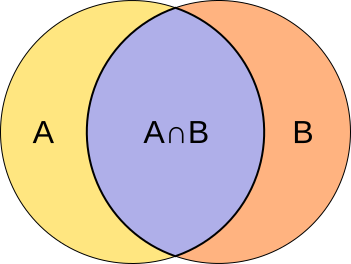
\includegraphics[scale=0.5]{intersection}
%\end{figure}
%
%\begin{figure}[h]
%	\caption{Union of two sets A and B \cite{wikipedia:union}}
%	\centering
%	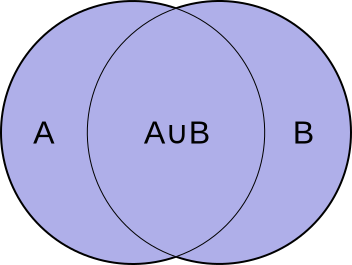
\includegraphics[scale=0.5]{union}
%\end{figure}
%
%\begin{equation}
%distance(set_1,set_2) = \frac{set_1 \cap set_2}{set_1 \cup set_2}
%\end{equation}
%
%For binary data the Jaccard index is the form of
%
%\begin{equation}
%J = \frac{M_{11}}{M_{01} + M_{10} + M_{11}},
%\end{equation}
%
%where
%
%$M_{11}$ is the total number of attributes where item1 and item2 both have a value of 1
%
%$M_{01}$ is the total number of attributes where item1 has the value of 0 and item2 has the value of 1
%
%$M_{10}$ is the total number of attributes where item1 has the value of 1 and item2 has the value of 0
%
%\begin{equation*}
%J([a',b')
%\end{equation*}
%
%\begin{equation*}
%J([0.5, 0.25, 1, 1, 0.67, 1],[0, 1, 0.29, 0.33, 0.5, 0])
%\end{equation*}
%
%Union $a' \cup b'  = \left\lbrace  0, 0.25, 0.29, 0.33, 0.5, 0.67, 1 \right\rbrace  $
%
%Intersection is  $a' \cap b'  = \left\lbrace 0.5, 1 \right\rbrace  $
%
%Jaccard index is then
%
%\begin{equation*}
%\frac{2}{7} = 0.286
%\end{equation*}
%
%\subsection{Cosine similarity}
%
%Cosine similarity is a measure of similarity between two vectors of an inner product space that measures the cosine of the angle between them. \cite{gorakala15}
%
%good in item based collaborative filtering ICBF \cite{gorakala15}
%
%Given to vectors of attributes, A and B, the cosine similarity can be calculated using dot product and magnitude as
%
%\begin{equation}
%similarity = cos(\theta) = \frac{A \cdot B}{||A||||B||} = \frac{\sum_{i=1}^{n}A_iB_i}{\sqrt{\sum_{i=1}^{n}A_i^2}\sqrt{\sum_{i=1}^{n}B_i^2}}
%\end{equation}
%
%For our example vectors, a' and b', the cosine similarity is
%
%\begin{equation*}
%similarity = \frac{\sum_{i=1}^{6}{a'}_i{b'}_i}{\sqrt{\sum_{i=1}^{6}{a'}_i^2}\sqrt{\sum_{i=1}^{6}{b'}_i^2}}
%\end{equation*}
%
%\begin{equation*}
%= \frac{(0.5 * 0) + (0.25 * 1) + (1 * 0.29) + (1 * 0.33) + (0.67 * 0.5) + (1 * 0)}{\sqrt{0.5� + 0.25� + 1� + 1� + 0.67� + 1�}\sqrt{0� + 1� + 0.29� + 0.33� + 0.5� + 0�}}
%\end{equation*}
%
%\begin{equation*}
%= \frac{0 + 0.25 + 0.29 + 0.33 + 0.335 + 0}{\sqrt{0.25 + 0.0625 + 1 + 1 + 0,449 + 1}\sqrt{0 + 1 + 0.0841 + 0.109 + 0.25 + 0}}
%\end{equation*}
%
%\begin{equation*}
%= \frac{1.205}{1.939 * 1.201}
%\end{equation*}
%
%\begin{equation*}
%= \frac{1.205}{2.329}
%\end{equation*}
%
%\begin{equation*}
%= 0.517 = 0.52
%\end{equation*}
%
%\subsection{Pearson product-moment correlation coefficient}
%
%Similarity between two items can also be given by the correlation existing
%between their attributes. Pearson correlation coefficient is a popular correlation coefficient calculated between two variables as the covariance of the two variables divided by the product of their standard deviations. \cite{gorakala15}
%
%
%Pearson correlation is correlation, whereas the previous similarity metrics give the actual score for similarity or distance. Therefore a straight comparison between these is not useful.
%
%Pearson correlation is invariant to adding constants.
%
%Pearson correlation is given by
%
%\begin{equation}
%\rho_{X,Y} = \frac{cov(X,Y)}{\sigma_X \sigma_Y}
%\end{equation}
%
%Wins others in user based collaborative filtering \cite{gorakala15} ??
%
%Covariance is given by
%
%\begin{equation}
%cov(X,Y) = \sum_{i = 1}^{n}(x_i-\overline{x})(y_i-\overline{y})
%\end{equation}
%
%Standard deviation is given by
%
%\begin{equation}
%\sigma_X = \sqrt{\sum_{i = 1}^{n}(x_i - \overline{x})�}
%\end{equation}
%
%where $\overline{x}$ (and $\overline{y}$) is the mean and is given by $\overline{x} = \frac{1}{n}\sum_{i = 1}^{n}x_i$
%
%\begin{equation}
%\rho_{x,y} = \frac{\sum_{i = 1}^{n}(x_i-\overline{x})(y_i-\overline{y})}{\sqrt{\sum_{i = 1}^{n}(x_i - \overline{x})�}\sqrt{\sum_{i = 1}^{n}(y_i - \overline{y})�}}
%\end{equation}
%
%\begin{equation*}
%= -0.60
%\end{equation*}
%
%Result is negative which implies that the values of b are decreasing when the values of a are increasing.
%
%\subsection{Others}
%
%Several other similarity measures exist. However, due to their inpopularity they are not described in detail.
%
%Hamming distance can be used to find the distance between two strings of equal length. For example block codes.
%
%Levenshtein distance is a string metric for calculating the difference between two sequences. Unlike Hamming distance, it takes into account strings of varying lengths thus being more suitable for spell checkers.
%
%Damerau?Levenshtein distance allows insertion, deletion, substitution.
%
%\subsection{Summary}
%6
%The following table prevents the previously calculated similarity results.
%
%\begin{center}
%	\begin{tabular}{ | l | c |}
%		\hline
%		\textbf{Measure} & Score \\ \hline
%		Euclidean distance & 0.37 \\ \hline
%		Jaccard index & 0.286 \\ \hline
%		Cosine distance & 0.52 \\ \hline
%		Pearson correlation & -0.60 \\ \hline
%	\end{tabular}
%	\captionof{table}{Similarity measures}
%\end{center}
%
%As seen from the table 3.2, cosine distance seems to be most suitable for the kind of data we are measuring. Pearson correlation does not provide a traditional score as it describes whether the values are relatively increasing or decreasing. Maybe it should be omitted from the comparison.

%\chapter{Data Processing}
%
%Solving a data analysis problem usually follows some set of steps that should to be executed in a specific order. This process is formally known as Knowledge Discovery in Databases (KDD). However, variations also exist in these definitions. Correctly performing these steps can significantly increase the effectiveness of the actual data mining task \cite{fayyad96}. Different definitions for solving a data mining task have been proposed, some are more abstract as in \cite[p. 39]{ricci11} while others dive more into details \cite{gorakala15} \cite{visa15} \cite{fayyad96}. The following section describes the KDD process and refines the tasks in the scope of this thesis.
%
%\section{Knowledge discovery in databases}
%
%The term knowledge discovery in databases refers to relatively older technologies such as data warehousing and traditional databases which hold the information. Currently the name is changing into something else since the data sources are varying (streaming, cloud, PaaS, SaaS, NoSQL, Graph databases).
%
%The following KDD process is aggregated from \cite{fayyad96} \cite{gorakala15} \cite{ricci11} and \cite{visa15}. The main form of the process comes from \cite{fayyad96} and \cite{visa15} and it is enhanced with more specific information from \cite{gorakala15} and \cite{ricci11}.
%
%The first step is to identify the business problem that is to be solved \cite{gorakala15} and to learn the application domain which refers to gathering relevant prior knowledge and studying the goals of application \cite{gorakala15} \cite{visa15} \cite{fayyad96}. Usually this is done with the help of a domain expert.
%
%Second step is to identify the data sources and data variables suitable for the analysis. \cite{gorakala15} \cite{visa15} \cite{fayyad96} In other other words, this step refers to selecting the data for the task.
%
%Third step is data cleaning and various preprocessing tasks such as identifying missing values, filling missing values, quantitative and qualitative variables and transformations. \cite{gorakala15} \cite{visa15} \cite{ricci11} \cite{fayyad96} This is usually the most time and effort consuming task of the KDD process. The third step also includes data transformation and reduction tasks such as finding useful features or reducing dimensionality \cite{visa15} \cite{fayyad96}. Data transformation is an preprocessing task in which numerical values can be normalized and usually this performed by normalizing the original values into the range of [0,1]. Data reduction refers to methods such as Principal Component Analysis (PCA), in which the data is projected into high dimensional feature space and ordered into principal components. PCA is discussed more in section 3.1.4.
%
%Fourth step is to choose the correct data mining method that matches with the goals of the KDD process. The method can be summarization, classification, regression, association or clustering \cite{visa15} \cite{fayyad96}. Choosing the mining algorithm and selecting methods for searching patterns \cite{visa15} \cite{fayyad96}.
%
%Fifth step is exploratory analysis to acquire better understanding of the data. Exploratory analysis includes tasks such as creating histograms \cite{gorakala15} or performing basic statistics such as mean, median, modes, variances, standard deviations, correlation among the variables and covariance to understand the nature of the data \cite{gorakala15}. 
%
%Sixth step is Data mining: search for patterns of interest \cite{visa15} \cite{fayyad96} This step has received the most attention in the literature thus being the best known component of KDD. The data mining step can include tasks such as dividing the data into training and testing datasets, running a model using machine-learning algorithms with training datasets, using cross-validation techniques. \cite{gorakala15}
%
%Seventh step is interpreting the mined patterns, possibly returning to any of steps 1 through 7 for further iteration. This step can also involve visualization of the extracted patterns and models or visualization of the data given the extracted models \cite{fayyad96} Validating the model using the test data to evaluate the model on the new data. If needed, improve the model based on the results of the validation step. \cite{gorakala15} Pattern evaluation and knowledge presentation such as visualization, transformation and removing redundant patterns. \cite{visa15}
%
%Eighth step is acting on the discovered knowledge. Using the information on other systems or just informing the interest parties about the results \cite{fayyad96} \cite{visa15}.  Result Interpretation \cite{ricci11} \cite{gorakala15} suggests that the last step is to deploy the model for real-time predictions.
%
%The KDD process can include several iteration loops between any two steps \cite{fayyad96}. The following subsections will present the steps to solve the data analysis problem.
%
%\subsection{Business problem}
%
%Products need to be recommended. Recommendation engine should be built. Scala and Spark was meant to be learnt.
%
%\subsection{Data sources}
%
%Initially the plan was to get the data from APIs or exporting dumps from mongodb. The main data sources are two NodeJS scripts that generate users and products (smartphones).
%
%\subsection{Cleaning and preprocessing}
%
%As the project moved forward, quite many preprocessing steps were required. Most of them have no actual role in the final recommendation engine, but they were part of the steps that were taken and which lead to the final recommendation engine.
%
%Data from APIs so it is in JSON, might contain missing values -> needs to be filled somehow
%
%The first received dataset was JSON dump data which was exported from MongoDB, it needed to be cleaned a lot even before it was valid JSON and it could be imported to RStudio where I made the preprocessing, commas were missing between the objects, NumberInt(), NumberLong(), IsoDate() definitions in the properties.
%
%BEFORE AFTER EXAMPLE OF THE DATA ?
%
%Better would be to read directly from MongoDB as it is possible with spark, it was working nicely. This was an experiment where data was imported to a local mongodb instance the cleaned and also generated data and read it directly with Spark.
%
%Actual preprocessing in RStudio with R. Removing unneeded data, such as infoInOtherLanguages etc. Cleaning NA and NULL values into "" or depending on the data what suits in the context. This took quite a lot of time actually, no use in the end.
%
%After preprocessing export data from RStudio -> import it into NodeJS app which converts the data into ndjs format so that it can be imported into spark.
%
%Also it turned out that it was easier to export data from RStudio after cleaning into .csv format since Spark was able to read that easily. Later was revealed that MongoDB can also export data as csv.
%
%In the end, actual cleaning was not required since data is generated and in good form.
%
%Preprocessing needed before feeding it to the algorithm (normalization, cosine similarity, build an array of Rating objects). Spark has also a cosine similarity algorithm of its own, DIMSUM, which was developed and released to Spark by Twitter. Developers at Twitter were able to reduce 40 percents of computation time with the help of smart sampling of the data set.
%
%\subsection{Selection of method}
%
%Spark currently supports only ALS algorithm for collaborative filtering. Rather than selecting the method, the dataset needed to be crafted to suit the available method.
%
%\subsection{Exploratory analysis}
%
%Maybe unneeded since the data is generated, but we can still analyze it a bit. Min Max values for each feature are decided, then random sampling assigns the value between these min and max values.
%
%\subsection{Data mining}
%
%The dataset was divided into three parts: training, testing and validation. Machine Learning algorithm, ALS in this case, was run with Spark against the training dataset.
%
%\subsection{Interpreting mined patterns}
%
%As the step states, the dataset (the generator scripts) were re visited in order to produce better products. This time the products were made to be smartphones instead of mobile subscriptions. Smartphones have more meaningful attributes.
%
%\subsection{Using the knowledge}
%
%At least the results can be inspected.

\chapter{Apache Spark}

- Driver

- Executor

Apache Spark is an open source framework that combines an engine for distributing programs across clusters of machines with an elegant model for writing programs. \cite{ryza15} It provides high-level APIs in Java, Scala, Python and R.

Spark can be introduced more easily by describing its predecessor, MapReduce, and the advantages it offers. MapReduce offered a simple model for writing programs that could execute in parallel across hundreds of machines. MapReduce achieves nearly linear scalability as the data size increases. The execution time is maintained by adding more computers to handle the task.

Spark preserves MapReduce's linear scalability and fault tolerance while extending it in three important ways. In MapReduce the intermediate results between the map and reduce tasks must be written into memory where as Spark is able to pass the results directly to the next step in the pipeline. Spark also treats the developers better by offering a rich set of transformations which enables users to represent complex pipelines in a few lines of code. (EXAMPLE?) Spark also introduces in-memory processing by introducing Resilient Distributed Dataset (RDD) abstraction which offers a way for developers to materialize any step in a processing pipeline and store it into memory. This means that future steps do not need to calculate the previous results again. Previously this kind of feature has not been available within distributed processing engines. \cite{ryza15}

Spark programs can be written using Java, Scala, Python or R. However, using Spark with Scala instead of Java, Python or R has a couple of advantages to it. Performance overhead is reduced, since tasks such as transferring data across different layers or performing transformations for data may result in weaker performance. Spark is written with Scala, which denotes that user has always access to latest and greatest features of the framework. Spark philosophy is easier to understand when Spark is used with the language it was built with. There is still one, maybe the biggest benefit of using Scala with Spark, and it is the developing experience that comes with the fact that user is using the same language for everything. Importing data from database, data manipulation, shipping the code into clusters. \cite{ryza15}

Spark is shipped with a read eval print loop (REPL). Usually when a application developed in REPL has matured enough, it is a good idea to move it into a compiled library (JAR). This way it is possible to prevent code and results from disappearing.

\section{Resilient Distributed Dataset (RDD)}

RDD is an abstraction for a collection of objects in spark that can be distributed across multiple machines in a cluster. When a new RDD is created, nothing is actually done, it means that spark knows where the data is when the time comes to do something with it.

RDD can be created in two ways: parallelizing an existing collection in the driver program or referencing an external dataset in an external storage system, such as a shared filesystem, HDFS, HBase or any data source offering a Hadoop InputFormat.?? \cite{spark-programming-guide}

\section{Dataset API}

Dataset, DS, is the replacement for RDD in Spark.

\section{Matrix Factorization}

Matrix factorization denotes a task in which a matrix is decomposed into a product of matrices. There are many different matrix decompositions. The following chapter will describe matrix factorization in general and the Alternating Least Squares algorithm which is the matrix factorization algorithm that is implemented in Spark. It is based on same idea as Netflix prize winner, matrix factorization models.

Matrix factorization belongs to a vast class of algorithms called latent-factor
models. Latent-factor models try to explain observed interactions between a large number of users and products through a relatively small number of unobserved, underlying reasons. For example, they can try to explain why people would buy a particular album out of endless possibilities by describing users and albums in terms of tastes which are not directly available as data. \cite{ryza15} A latent factor is not available for direct observation. For example health of a human being is a latent factor. Health can not be observed as a variable such as blood pressure.

\begin{figure}[h]
	\caption{Matrix factorization \cite{ryza15}}
	\centering
	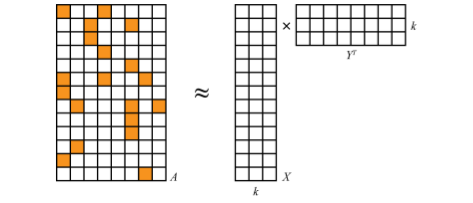
\includegraphics[scale=0.8]{matrix_factorization}
\end{figure}

Matrix factorization algorithms treat the user and product data as if it was a large matrix A. Each entry in row i and column j represents a rating the user has given to a specific product. \cite{ryza15}

Usually $A$ is sparse, which denotes that most of the entries of $A$ are 0. This is due to the fact that usually only a few of all the possible user-product combinations exist.

Matrix factorization models factor $A$ as the matrix product of two smaller matrices, $X$ and $Y$, which are quite tiny. Since $A$ has many rows and columns, both of them have many rows, but both have just a few columns $(k)$. The $k$ columns match to the latent factors that are being used to explain the interactions of the data. The factorization can only be approximate because $k$ is small. \cite{ryza15}

The standard approach to matrix factorization based collaborative filtering treats the entries in the user-product matrix as explicit preferences given by the user to the product, for example users giving ratings to movies. Implicit data denotes for example page views or a value representing if a user has listened to a artist. Explicit data means actual ratings that a user has given to a product. Spark ALS can handle both implicit and explicit data. \cite{spark14} \cite{ryza15}

Usually many real-world use cases have access only to implicit feedback data such as views, clicks, purchases, likes or shares. However, instead of trying to model the matrix of ratings directly, the approach in Spark MLlib treats the data as numbers representing the strength of the observations such as the number of clicks, or the cumulative duration someone spent viewing a movie. Instead of explicit ratings, these numbers are related to the level of confidence in observed user preferences. Based on this data, the model tries to find latent factors that can be used to predict the expected preference of a user for an item. \cite{spark14}

Sometimes these algorithms are referred to as matrix completion algorithms. This is because the original matrix $A$ may be sparse while the product $XY^T$ is dense. Hence, the product is only an approximation of $A$. \cite{ryza15} In this thesis, the original user-item matrix $A$ is actually very dense since we have a value in every entry of the matrix.

\subsection{Alternatig Least Squares (ALS)}

Collaborative filtering is commonly used for recommender systems. These techniques aim to fill in the missing entries of a user-item association matrix. Spark MLlib currently supports model-based collaborative filtering, in which users and products are described by a small set of latent factors that can be used to predict missing entries. Spark MLlib uses the Alternating Least Squares (ALS) algorithm to learn these latent factors. \cite{spark14}

Spark ALS attempts to estimate the ratings matrix A as the product of two lower-rank matrices, $X$ and $Y$. \cite{als14}

\begin{equation}
A = XY^T
\end{equation}

Typically these approximations are refered to as factor matrices. The general approach is iterative. During each iteration, one of the factor matrices is held constant, while the other is solved for using least squares. The newly-solved factor matrix is then held constant while solving for the other factor matrix. \cite{als14} Spark ALS enables massive parallelization since it can be done separately, it can be done in parallel which is an excellent feature for a large-scale computation algorithm. \cite{ryza15}

Spark ALS is a blocked implementation of the ALS factorization algorithm. Idea is to group the two sets of factors, referred to as $users$ and $products$, into blocks. Grouping is followed by reducing communication by only sending one copy of each user vector to each product block on each iteration. Only those user feature vectors are sent that are needed by the the product blocks. Reduced communication is achieved by precomputing some information about the ratings matrix to determine the out-links of each user and in-links of each product. Out-link denotes those blocks of products that the user will contribute to. In-link refers to the feature vectors that each product receives from each user block they depend on. This allows to send only an array of feature vectors between each user block and product block. Consequently the product block will find the users' ratings and update the products based on these messages. \cite{als14}

Essentially, instead of finding the low-rank approximations to the rating matrix $A$, it finds the approximations for a preference matrix $P$ where the elements of $P$ are 1 when r > 0 and 0 when r <= 0. The ratings then act as confidence values related to strength of indicated user preferences rather than explicit ratings given to items. \cite{als14}

\begin{equation}
A_iY(Y^T Y)^{-1} = X_i
\end{equation}

Alternating Least Squares operates by rotating between fixing one of the unknowns $u_i$ or $v_j$. While the other is fixed the other can be computed by solving the least-squares problem. This approach is useful because it turns the previous non-convex problem into a quadratic that can be solved optimally \cite{aberger14}. A general description of the algorithm for ALS for collaborative filtering taken from \cite{aberger14} is as follows:

\begin{lstlisting}[caption=Alternating Least Squares algorithm \cite{aberger14}]

1. Initialize matrix V by assigning the average rating for that movie as the first row, and small random numbers for the remaining entries.

2. Fix V, solve U by minimizing the RMSE function.

3. Fix U, solve V by minimizing the RMSE function.

4. Repeat Steps 2 and 3 until convergence.

\end{lstlisting}

Minimizing the Root Mean Square Error RMSE function denotes a task in which line is plotted. EXPLAIN RMSE.

\chapter{Implementation}

- MovieLens ml-latest-small dataset.

- What is MovieLens?


\chapter{Result}

\chapter{Evaluation}
\label{ch:concl}

\section{Conclusion}

There are a number of possible implementations for a recommendation engine. This was selected because Apache Spark could be a good tool to know in future and in addition learning Scala programming was another thing that was considered.

Existing recommendation or analytic engines should be evaluated before making a decision about the recommendation engine.

In the end the most difficult thing was to find the right approach for this task. By trial and error the right combination of technologies and an actual working example was found.

\section{Future work}

Actual parallelization?

Lately, a number of service providers, like Telegram and Microsoft, have started to introduce bot frameworks for their services. A bot is a web service that uses a conversational format to interact with users. Users can start conversations with the bot from any channel the bot is configured to work on. Conversations can be designed to be freeform, natural language interactions or more guided ones where the user is provided choices or actions. It is possible to utilize simple text strings or something more complex such as rich cards that contain text, images, and action buttons. \cite{bots16}

Already for a long time, companies have had some sort of SMS that have been accepting feedback from customer or ordering a new data package for you mobile subscription. IRC channel bots have been around even longer. Idea is not new but now there are popular platforms for the bots. As any other idea, also a recommendation engine could be implemented in a way that it can be used via a bot. For example ElasticSearch forms a RESTful API so a bot could simply place queries against the API.

%
% The bibliography, i.e the list of references (3 options available)
%
\newpage

\renewcommand{\bibname}{Bibliography}     % Otherwise bilingual babel uses Finnish ``Kirjallisutta''. Strange...
%\renewcommand{\bibname}{L�hteet}         % Set Finnish header, remove this if using English
%\addcontentsline{toc}{chapter}{L�hteet}  % Include this in TOC
\addcontentsline{toc}{chapter}{\bibname}  % Include this in TOC

\bibliographystyle{IEEEtranS}

\bibliography{thesis_refs}    % Insert {author,title,year...} info of your reference
\markboth{\bibname}{\bibname} % Set page header

\end{document}

